%------------------------------------
\chapter{Centrifugal Instability}
%------------------------------------
%------------------------------------
\section{Q. 3.1: The Oscillations of a Rotating Column of Liquid - by PA:}
%------------------------------------
Eliminating $u, v, w$ from the linearized perturbation equations (see \cite{drazin2004hydrodynamic} for details), we obtain the following equation and boundary conditions for the pressure perturbation  $\varpi$, where $p/\rho = \varpi e^{st + i(m\theta + k z)}$. In this problem $R_{1}=0$ and $R_{2}=R_{0}$. 

\begin{align}\label{eq:3_1_pressure_perturbation}
 \begin{split}
    \left(D_{*}D - \frac{m^{2}}{r^{2}} \right)\varpi &= k^{2}\left( 1 + \frac{4\Omega^{2}}{\gamma^{2}}\right)\\
    D\varpi + \frac{2im\Omega}{\gamma r} \varpi &= 0 \textrm{ at } r = R_{1}, r=R_{2} 
 \end{split}
\end{align}
where $D = d/dr, D_{*} = d/dr + 1/r$ and $\gamma = s + i m \Omega$. 

We rescale $r = \tilde{r}/R_{2}$ and let $a = kR_{2}$ to obtain
\begin{equation}\label{eq:3_1_bessel}
 \frac{d^{2}\varpi}{d\tilde{r}^{2}} + \frac{1}{\tilde{r}}\frac{d\varpi}{d\tilde{r}} + \left(-a^{2}\left( 1 + \frac{4\Omega^{2}}{\gamma^{2}}\right) - \frac{m^{2}}{\tilde{r}^{2}} \right)\varpi = 0
\end{equation}

This is the standard Bessel equation with solutions $\varpi(r) = A J_{m}(\alpha \tilde{r}) + B Y_{m}(\alpha \tilde{r})$. For regularity at $r=0$, we have $B = 0$. Here 
\begin{equation}\label{eq:3_1_alpha}
\boxed{\alpha^{2} = -a^{2}\left( 1 + \frac{4\Omega^{2}}{\gamma^{2}}\right)}. 
\end{equation}

Rescaling back to the original co-ordinates $r$, 
$\boxed{\varpi(r) = AJ_{m}(\alpha r/R_{2}) = AJ_{m}(\alpha r/R_{0})}$. 

The boundary condition applied at $r = R_{0}$ then implies that $\alpha$ must satisfy
\begin{equation}\label{eq:3_1_bc}
 \alpha J'_{m}(\alpha) + \frac{2im\Omega}{\gamma} J_{m}(\alpha) = 0.
\end{equation}

But from Eqn. (\ref{eq:3_1_alpha}), 
\begin{equation}\label{eq:3_1_alpha_inverted}
 \frac{2i\Omega}{\gamma} = \pm \sqrt{1 + \alpha^{2}/a^{2}} 
\end{equation}

Substituting Eqn.(\ref{eq:3_1_alpha_inverted}) into Eqn.(\ref{eq:3_1_bc}), $\alpha$ should be a root of the following equation:
\begin{equation}
 \alpha J'_{m}(\alpha) \pm m (1 +  \alpha^{2}/a^{2})^{1/2} J_{m}(\alpha) = 0
\end{equation}

Also, from Eqn.(\ref{eq:3_1_alpha_inverted}) and using the fact that $\gamma = s + im$, the frequencies of oscillations are given by

\begin{equation}\label{eq:3_1_freq_of_oscillations}
 \boxed{\frac{s}{\Omega_{0}} = \pm \frac{2i}{(1 +  \alpha^{2}/a^{2})^{1/2}} - im}.
\end{equation}

For the graphs of $is/\Omega_{0}$ Pulkit Dubey (PD) has a mathematica code, which will be uploaded soon. Also, $\S 68$ of \cite{chandrasekhar1961hydrodynamic} goes through the same analysis and plots the dispersion relation as in Fig. (\ref{fig:rotating_col_dispersion_chandra}), where $\alpha_{m, j}$ is the $j^{th}$ zero of $J_{m}(x)$.

 \begin{figure}[H]
    \centering
    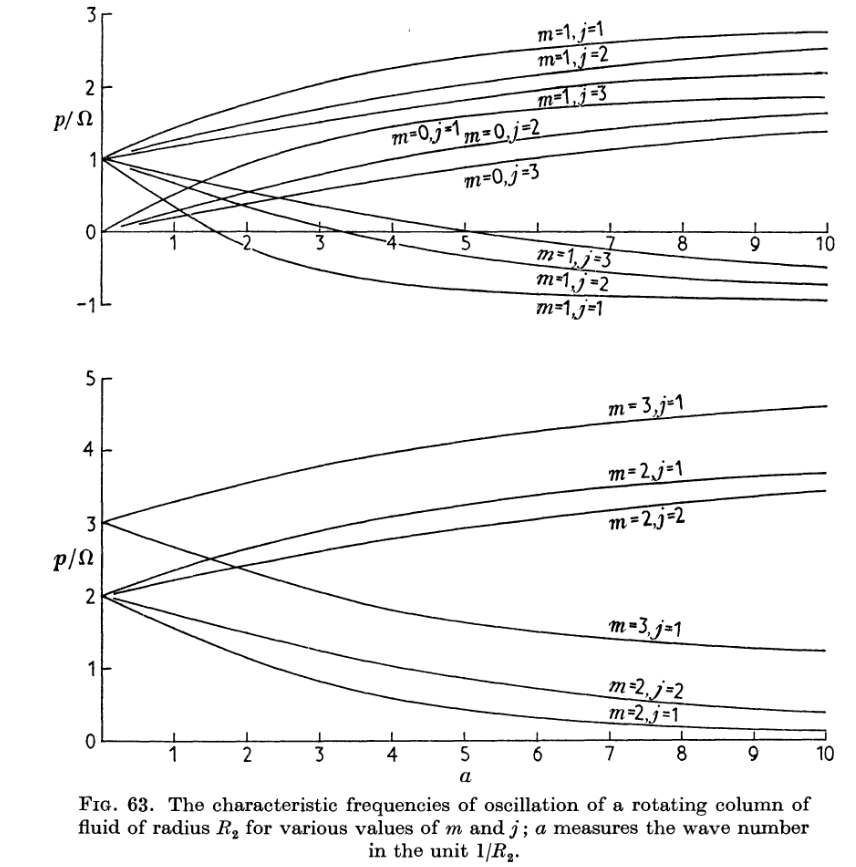
\includegraphics[scale = 0.4]{Figs/rotating_col_dispersion_chandra.png}
    \caption{Dispersion relation $is/\Omega_{0}$ vs. $a$, reproduced from \cite{chandrasekhar1961hydrodynamic}.}
    \label{fig:rotating_col_dispersion_chandra}
\end{figure}
%------------------------------------
\section{Q. 3.2: The analogue of Rayleigh's inflexion point theorem for two-dimensional disturbances of rotating and curved flows - by PA:}
%------------------------------------
As in sec. $\S 15.3$, we only consider $2d$, non-axisymmetric disturbances in the $\theta-z$ plane and define a stream-function $\psi'$ of the perturbation

\begin{equation}\label{eq:3_2_streamfunction}
 u'_{r} = \frac{1}{r}\frac{\partial \psi'}{\partial \theta} \textrm{, } u'_{\theta} = -\frac{\partial \psi'}{\partial r}. 
\end{equation}

We then perform a normal mode analysis on the perturbation streamfunction with $\psi'(r, \theta, t) = \phi(r) \exp{[st + i n \theta]}$, set $d/dz = 0$, eliminate pressure, to get
\begin{equation}\label{eq:3_2_phi}
 (s + i n \Omega)(D_{*}D - n^{2}/r^{2})\phi - inr^{-1}(DZ)\phi = 0,
\end{equation}
with $D = d/dr, D_{*} = d/dr + 1/r$ and $Z = r D\Omega + 2\Omega$ is the basic vorticity. 

Multiplying Eqn. \ref{eq:3_2_phi} by $r\phi^{*}/(s + i n \Omega)$, we obtain
\begin{equation}\label{eq:3_2_integrand}
 r\phi^{*}\left(D_{*}D - \frac{n^{2}}{r^{2}} \right)\phi - \frac{in DZ}{s+in\Omega}\phi \phi^{*} = 0
\end{equation}

Focusing on the $\int_{R_{1}}^{R_{2}} r\phi^{*}D_{*}D \phi dr$ term, 

\begin{align}
 \begin{split}
  \int r\phi^{*}D_{*}D \phi dr & = \int r\phi^{*}\left(\frac{d^{2} \phi}{dr^{2}} + \frac{1}{r}\frac{d\phi}{dr}\right)dr\\
%  
  & = r\phi^{*}\frac{d\phi}{dr} - \left[\int r \frac{d\phi^{*}}{dr}\frac{d\phi}{dr} dr+ \cancel{\int \phi^{*}\frac{d\phi}{dr} dr}\right] + \cancel{\int \phi^{*}\frac{d\phi}{dr} dr} 
 \end{split}
\end{align}

This gives
\begin{equation}\label{eq:3_2_integral}
 \int_{R_{1}}^{R_{2}} r \left\{ |D\phi|^{2} + \frac{n^{2}}{r^{2}}|\phi|^{2} + \frac{in(DZ)|\phi|^{2}}{s + in\Omega}\right\}dr = \left[ r \phi^{*}D\phi\right]_{R_{1}}^{R_{2}}
\end{equation}

Due to rigid cylinders, $\phi = \phi^{*} = 0$ at $R_{1}$ and $R_{2}$ and hence RHS vanishes. Note that
\begin{equation}
\frac{in(DZ)|\phi|^{2}}{s + in\Omega} = \frac{in(s - in\Omega)(DZ)|\phi|^{2}}{|s + in\Omega|^{2}} 
\end{equation}

For instability, we know $ s > 0$ must be satisfied. Taking the imaginary part of Eqn. (\ref{eq:3_2_integral}), we obtain the analogue of Rayleigh's inflexion point theorem for two-dimensional disturbances of rotating and curved flows:

\begin{equation}\label{eq:3_2_rotating_Rayleigh_inflexion}
 n\int_{R_{1}}^{R_{2}}\frac{(DZ)|\phi|^{2}}{|s + in\Omega|^{2}} dr = 0. 
\end{equation}

Eqn. (\ref{eq:3_2_rotating_Rayleigh_inflexion}) implies that the sign of $(DZ)$ must change at least once between $R_{1}$ and $R_{2}$ for an instability to occur (necessary condition, not sufficient). 
%------------------------------------
%------------------------------------
\section{Q. 3.3: Jump Conditions - by PA:}
%------------------------------------
We consider the inviscid problem with $2d$ non-axisymmetric disturbances (No variation in $z$, $d/dz = 0, k = 0$.). We also suppose $\Omega$ or $D\Omega$ are discontinuous at $R_{0}$. Let the perturbed interface be given by $ r = R_{0} + \xi$, where $\xi = \xi_{0}\exp{(st + in\theta)}$.

To obtain the first jump condition, we require the normal velocity (in this case $u$) to be continuous across the perturbed interface. 
\begin{equation}\label{eq:3_3_u_continuity}
 u|_{R_{0}} = \frac{Dr}{Dt} = \left.\frac{D\xi}{Dt}\right\vert_{R_{0}} = \frac{\partial \xi}{\partial t} + \Omega \frac{\partial \xi}{\partial \theta} = \xi_{0}(s + in\Omega) 
\end{equation}
to the first order in perturbation. 

From Eqn.($15.22$) of \cite{drazin2004hydrodynamic}, $u = inr^{-1}\phi$, giving

\begin{align}\label{eq:3_3_first_jump_cond}
\begin{split}
 & \frac{in\phi}{R_{0}} = \xi_{0}(s + in\Omega)\\
 & \Rightarrow \boxed{\Delta \left[\frac{in \phi}{s + in\Omega} \right] = 0}.
\end{split}
\end{align}

Where $\Delta f = f(R_{0}^{+}) - f({R_{0}^{-}})$ as defined in the problem.

To obtain the second jump condition, we have $\Delta [\textrm{total pressure}] = 0$.
\begin{align}
 \begin{split}
 \Delta \left[ P(R_{0}+\xi) + p'(R_{0}+\xi) \right] &= 0\\
 \Delta \left[\cancel{(R_{0})} + \xi \frac{dP}{dr} + p'(R_{0}) \right] & \approx 0\\
 \Delta \left[\xi_{0} \frac{dP}{dr} + \rho \varpi \right] & \approx 0\\
 \textrm{From Eqn.} & 15.22\\
 \varpi &= - \frac{r}{in}[(s + in\Omega)v + (D_{*}V)u]\\
 \varpi &= \frac{1}{in}[r(s + in\Omega)D\phi - inZ\phi]\\
 \xi_{0} &=\frac{u}{(s+in\Omega)} = \frac{in}{r}\frac{\phi}{(s+in\Omega)}\\
 \frac{1}{\rho}\frac{dP}{dr} & = \Omega^{2}r\\
 \Rightarrow \Delta[r(s + in\Omega)D\phi - inZ\phi - n^{2}\Omega^{2}\phi/(s+in\Omega)] & = 0 \textrm{ at } r = R_{0}. 
\end{split}
\end{align}
